\vfill
\pagebreak
\section{Annexes}

\subsection{Esquisse de l'Interface Mobile}

\subsubsection{Ecran d'accueil}
Cet écran présent le logo de la Societé COPEVUE et les champs pour l'autentification
de l'utilisateur.

\begin{figure}[!h] 
\begin{center}
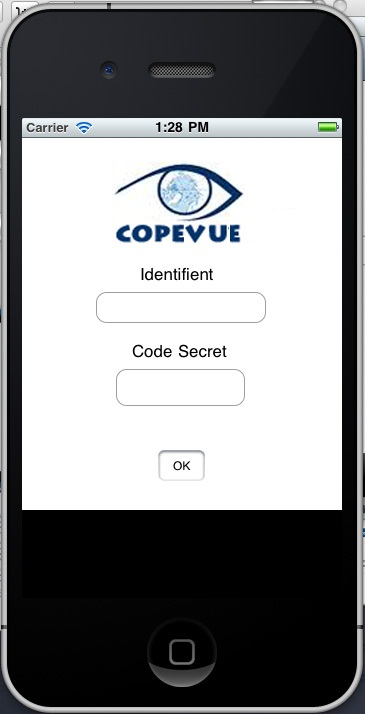
\includegraphics[width=6cm]{\PIXPATH/01.jpg} 
\end{center} 
\end{figure} 
\vfil
\pagebreak
\subsubsection{Ecran de Recherche}
Le champ texte permet de saisir le nom de l'objet de recherche.
Pour faire la recherche, l'application compte avec un multichoix qui nous permet de préciser les critères de recherche.

\begin{figure}[!h]
\begin{center}
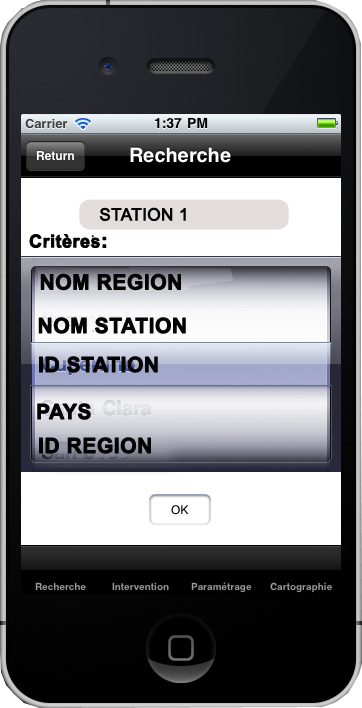
\includegraphics[width=6cm]{\PIXPATH/02.jpg}
\end{center} 
\end{figure} 

Le tab Bar nous permet de: Faire une recherche, Montrer la carte géographique, Faire une Intervention (demande Consultation), Faire des paramètrage. 
Si les critères sont mis, on valide avec le bouton "OK" pour commencer la recherche.

\vfil
\pagebreak
\subsubsection{Ecran Résultat de Recherche}
Ces écrans présent les résultats de recherches des stations.
Le bouton de retour permet de revenir à l'écran précédent.
Le tableau montre le résultat après avoir choisi les critères de recherche.

\begin{figure}[!h] 
\begin{center}
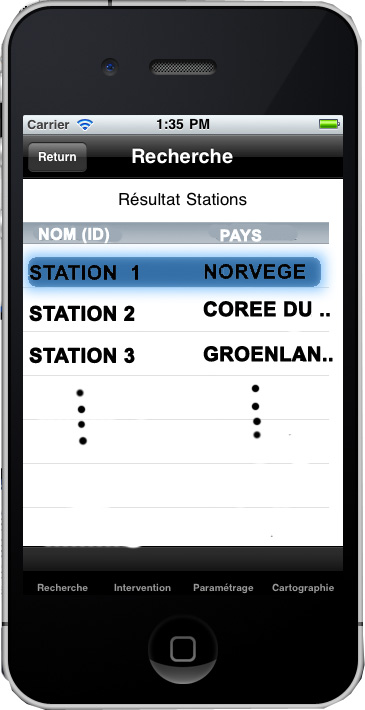
\includegraphics[width=6cm]{\PIXPATH/03.jpg} 
\end{center}
\end{figure} 

On peut faire double click sur la file qui nous intéresse pour avoir les informations générales tels que l'Id et le nom de station, le nombre de capteurs qui possède, le état de la station, date de modification, etc.

\begin{figure}[!htbp]
\begin{center}
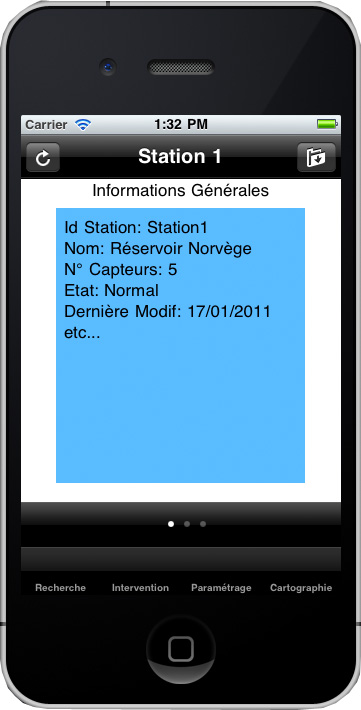
\includegraphics[width=6cm]{\PIXPATH/04.jpg}              
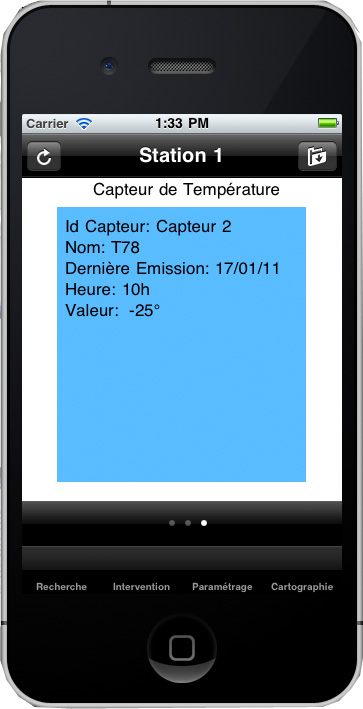
\includegraphics[width=6cm]{\PIXPATH/05.jpg}              
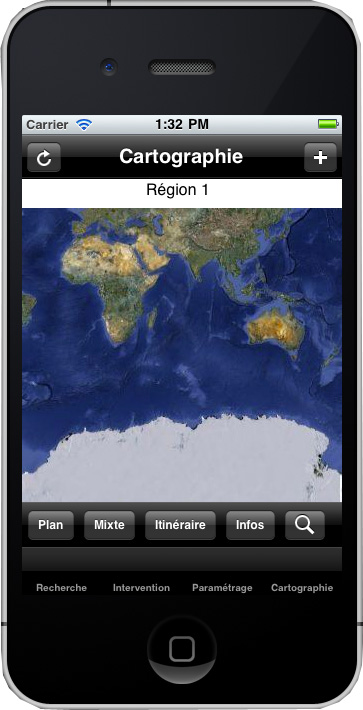
\includegraphics[width=6cm]{\PIXPATH/06.jpg}              
\end{center}
\end{figure} 
Le passage d'une information à l'autre s'effectue par balayage de l'écran de droite à gauche. 
Le bouton refresh permet de mettre à jour les informations avec les derniers données.
On peut accéder à la cartographie depuis cet écran, et nous affichera le map centré sur la station.

On peut aussi faire click sur Intervention pour faire un rapport.

\vfil
\pagebreak
\subsubsection{Ecran Emission d'un Rapport d'Intervention}
Cet écran nous permet d'émitir un rapport, on peut mettre le nom du rapport, la nature de l'intervention en indiquant si c'est une réparation, une maintenance, un remplissage, etc. 
On peut aussi faire des commentaires. Et enfin pour envoyer le rapport on click sur OK. L'application ajoutera automatiquement la date et le lieu du rapport.

\begin{figure}[!h] 
\begin{center}
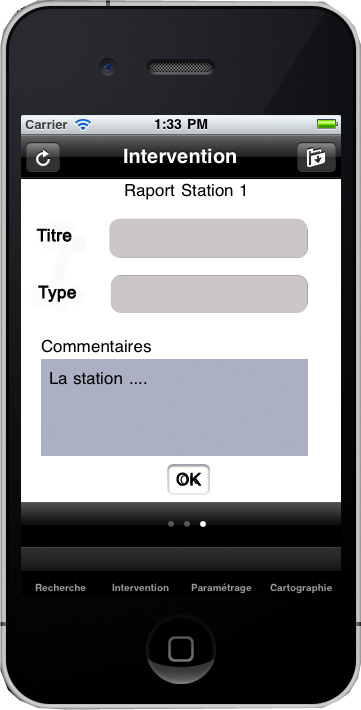
\includegraphics[width=6cm]{\PIXPATH/07.jpg}
\end{center}
\end{figure}

\vfil
\pagebreak
\subsubsection{Ecran Préférences}
Cet écran permet d'activer l'autologin. Le PDA gardera les données d'identifient et mot de passe.
On peut configurer aussi les critères de recherche, etc.
\begin{figure}[!h] 
\begin{center}
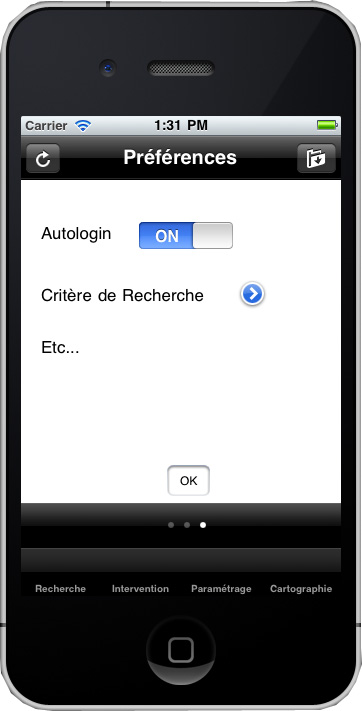
\includegraphics[width=6cm]{\PIXPATH/08.jpg}
\end{center}
\end{figure}


\end{document}
